\section{Computing Periodic Orbits} 
\label{sec:ComputingPeriodicOrbits}

\subsection{Families of Periodic Orbits}
The CR3BP admits infinitely many periodic orbits \cite{Poincare_1957}.
Many of these orbit families have been studied extensively and several have found practical applications in space mission design. 
In this work, we restrict our analysis to planar periodic orbits and illustrate how they can be computed numerically using differential correction. 
An initial condition $\boldsymbol{x}_0$ lies on a periodic orbit if there exists a time $T>0$ such that
\begin{equation*}
    \boldsymbol{\phi}(T,\boldsymbol{x}_0) =\boldsymbol{x}_0.
\end{equation*}
The smallest positive value of $T$ is called the period of the orbit.

\begin{figure*}[t!]
  \centering
  \begin{subfigure}[b]{0.32\linewidth}
    \centering
    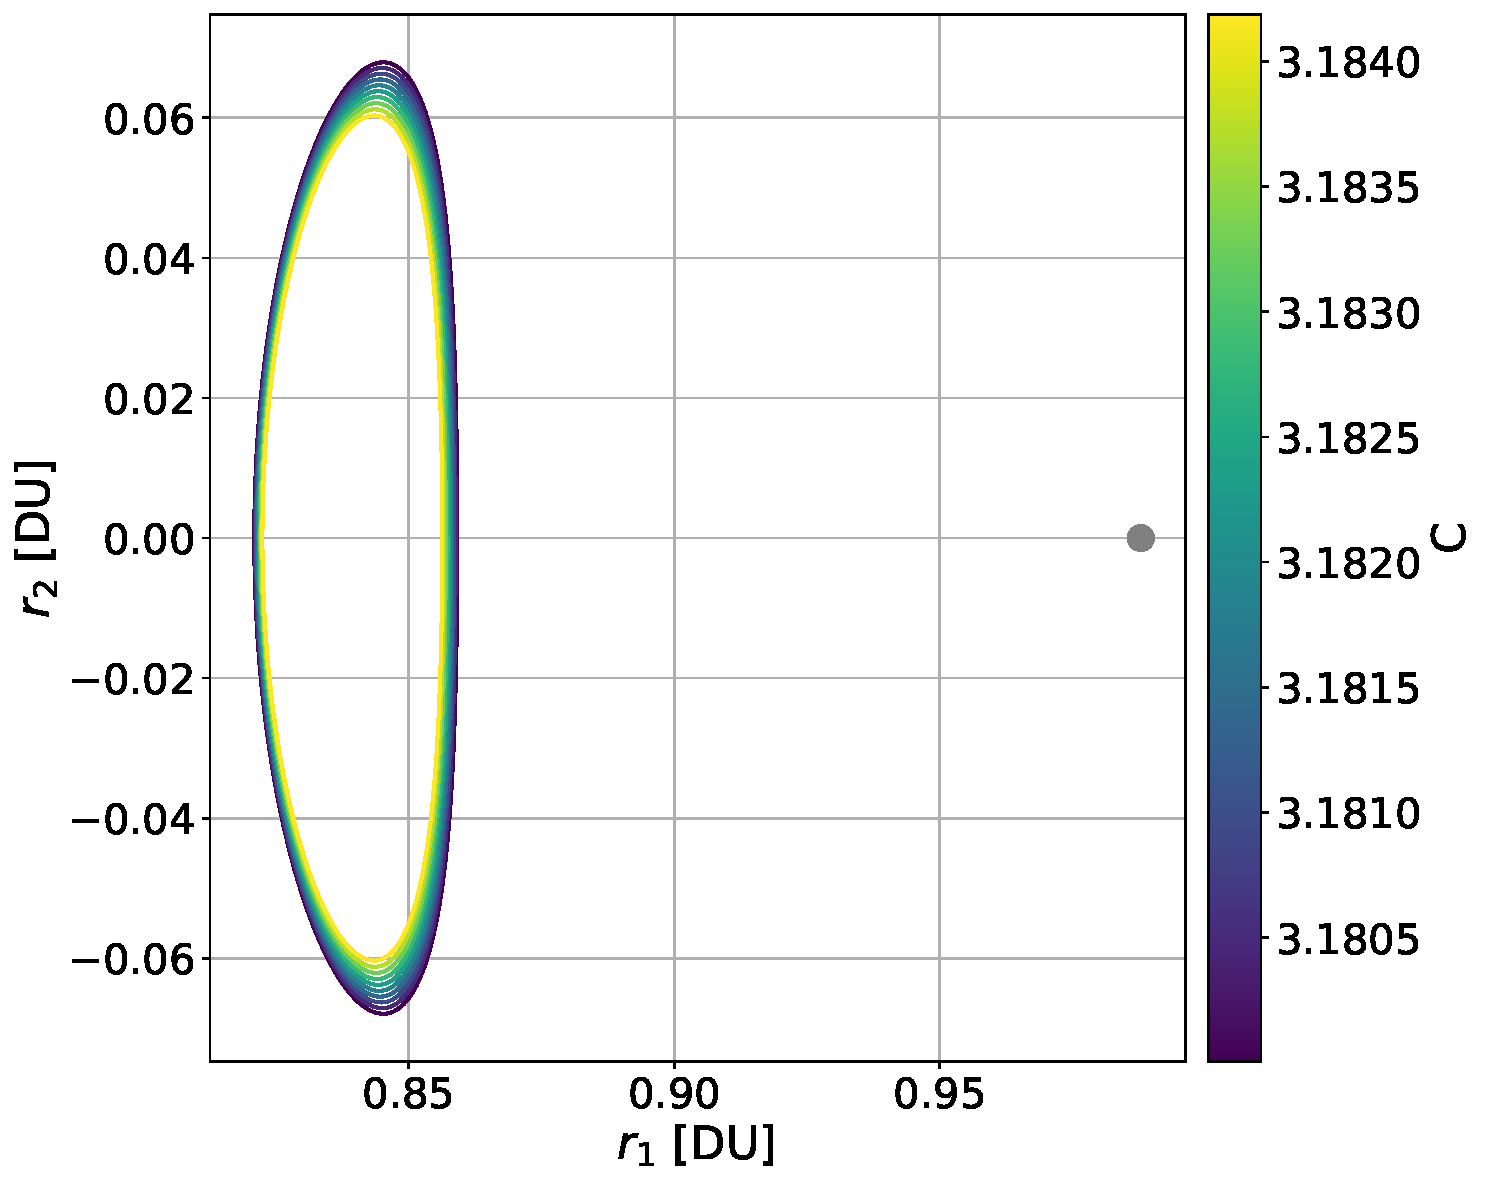
\includegraphics[width=\linewidth]{images/lyapunov_step20_E-1.584--1.586.pdf}
    \caption{Lyapunov}
    \label{fig:sub_a}
  \end{subfigure}
  \hfill
  \begin{subfigure}[b]{0.32\textwidth}
    \centering
    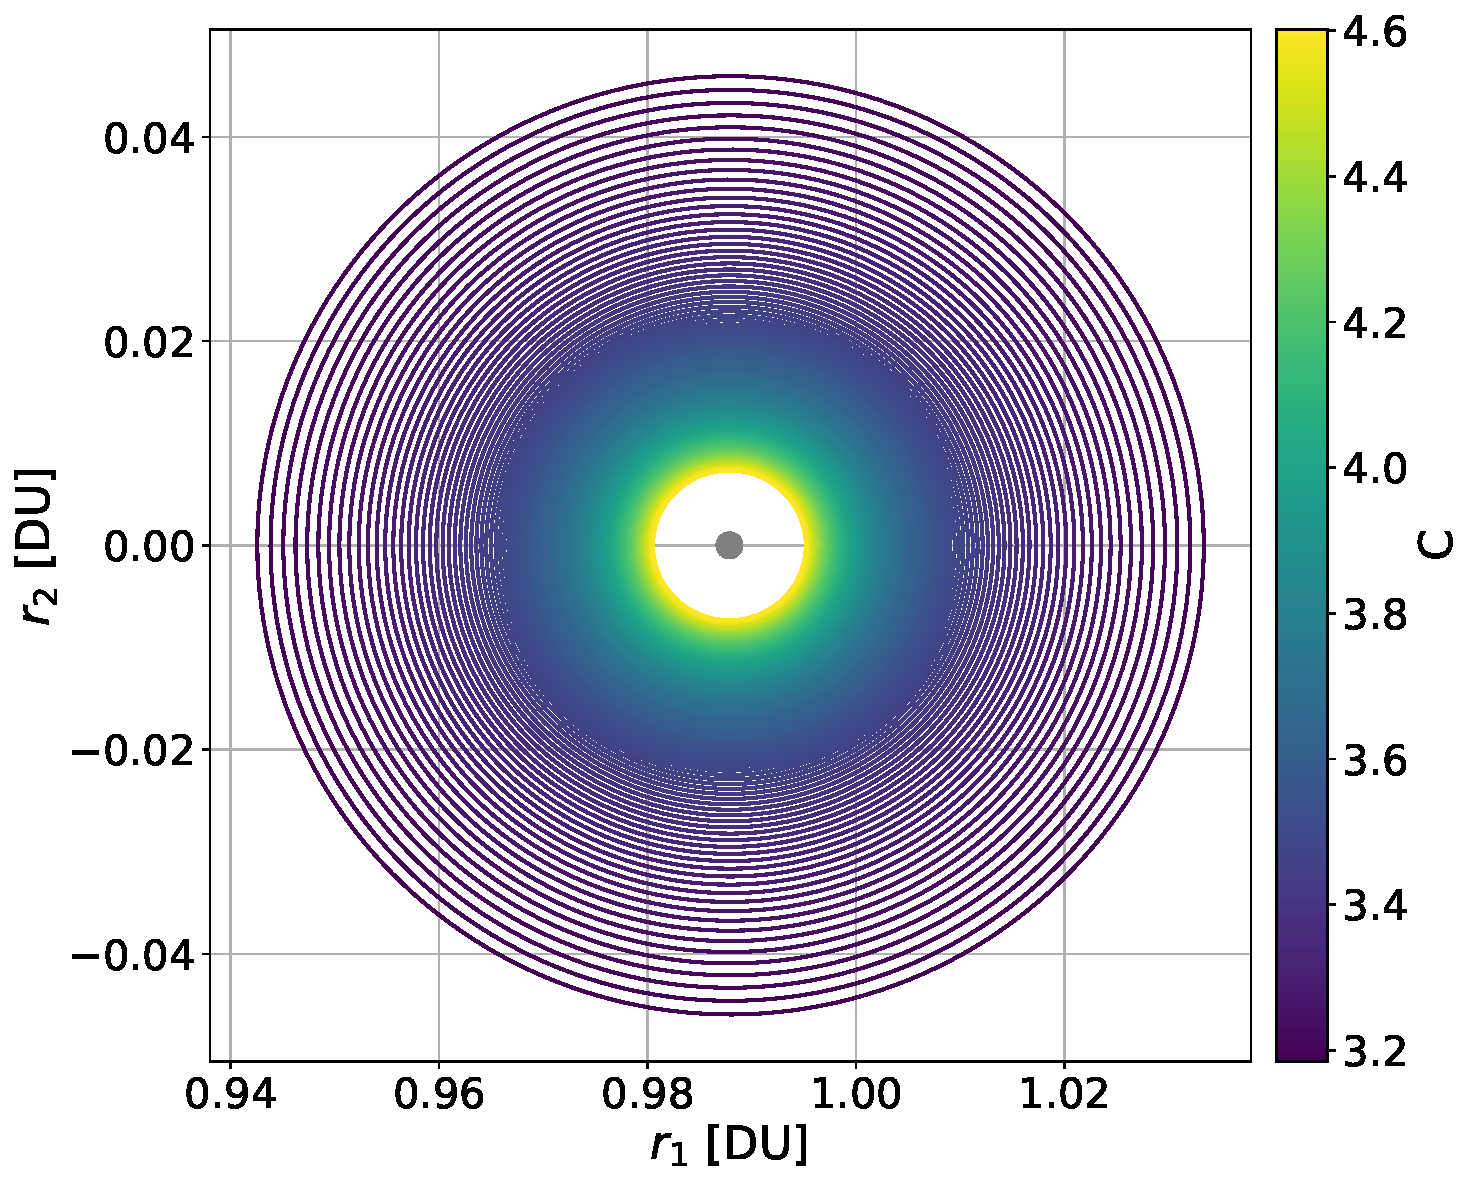
\includegraphics[width=\linewidth]{images/dros_step15_jacobimin3.172.pdf}
    \caption{DRO}
    \label{fig:sub_b}
  \end{subfigure}
  \hfill
  \begin{subfigure}[b]{0.32\textwidth}
    \centering
    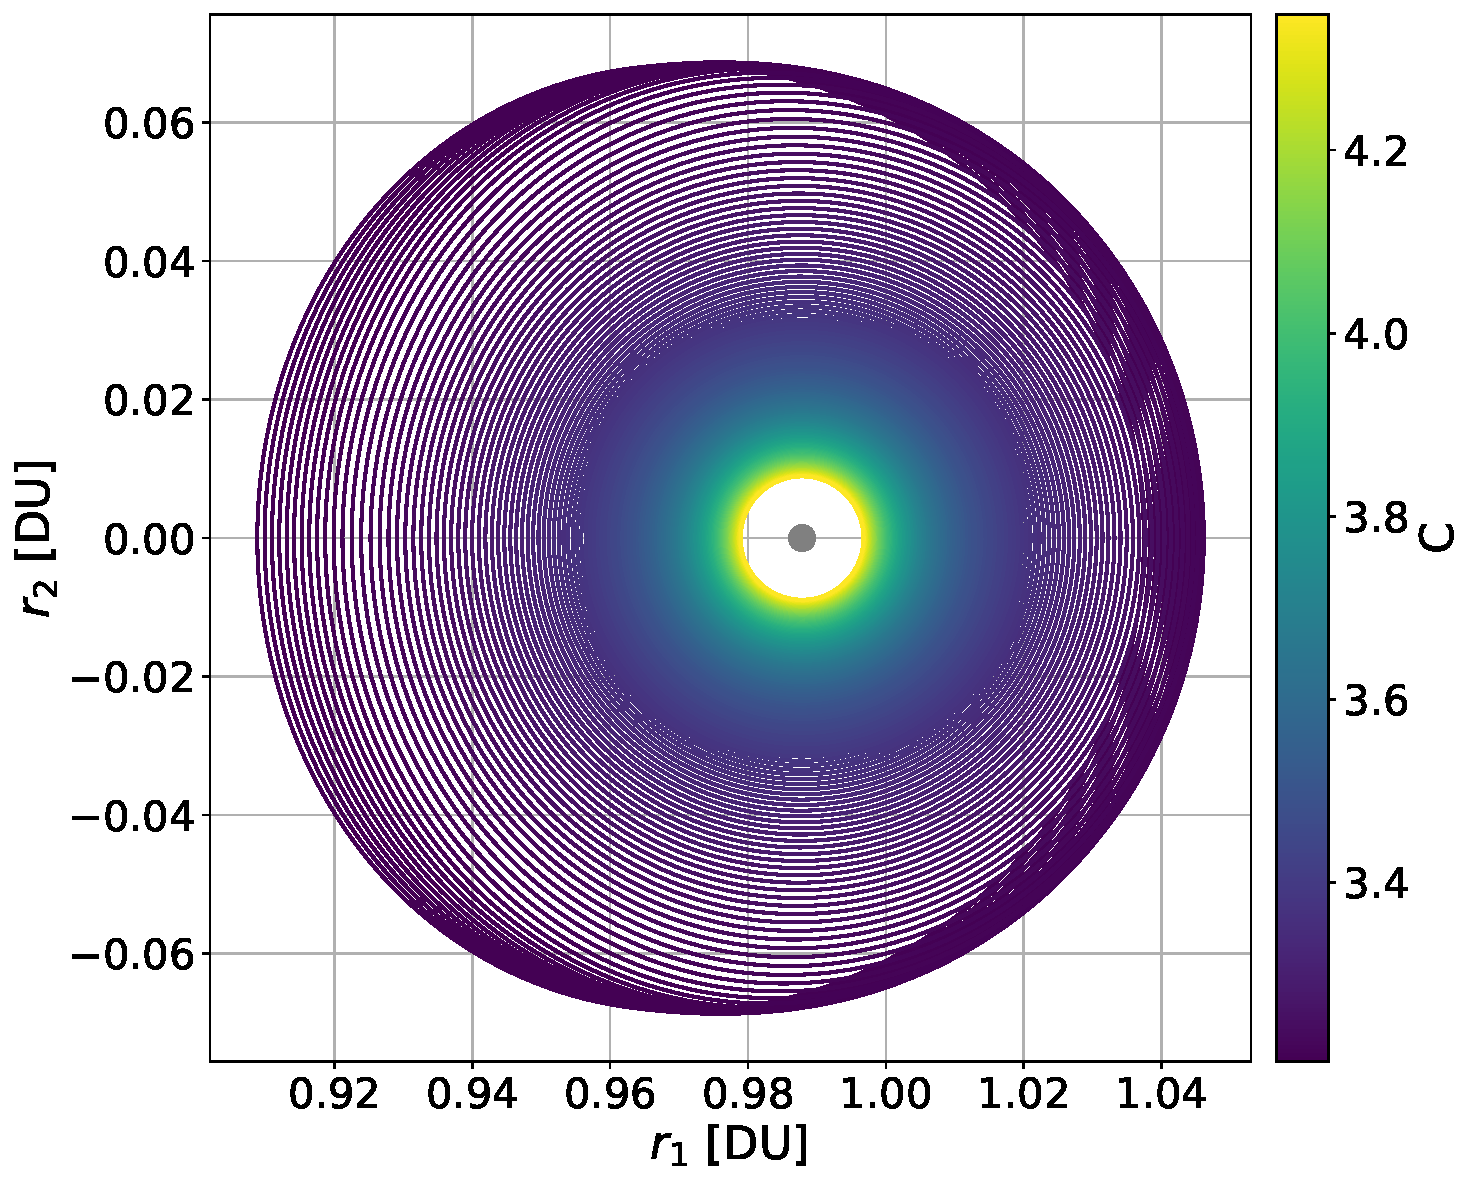
\includegraphics[width=\linewidth]{images/dpos_step15_jacobimin3.172.pdf}
    \caption{DPO}
    \label{fig:sub_c}
  \end{subfigure}
  \caption{Examples of different families of orbits in the lunar regime, shown in the $x,y$ plane of the CR3BP. Colours indicate the Jacobi constant for each orbit.}
  \label{fig:lunar_orbits}
\end{figure*}
Starting from an initial guess for the state $\boldsymbol{x}_0$, periodic orbits can be computed using a differential correction algorithm. \cref{fig:lunar_orbits} shows representative planar periodic orbits in the lunar region. 
These include Moon-centred orbit families, such as distant retrograde orbits (DROs) and distant prograde orbits (DPOs), as well as equilibrium-point-centred families, such as Lyapunov orbits.
\begin{figure*}[b!]
  \centering
  \begin{subfigure}[b]{0.32\linewidth}
    \centering
    \includegraphics[width=\linewidth]{images/resonant_7.0_1.0_retro_False_step20_jacobimin3.172.png}
    \caption{7:1 Prograde}
    \label{fig:suba}
  \end{subfigure}
  \hfill
  \begin{subfigure}[b]{0.32\textwidth}
    \centering
    \includegraphics[width=\linewidth]{images/resonant_9.0_2.0_retro_False_step20_jacobimin3.172.png}
    \caption{9:2 Prograde}
    \label{fig:subb}
  \end{subfigure}
  \hfill
  \begin{subfigure}[b]{0.32\textwidth}
    \centering
    \includegraphics[width=\linewidth]{images/resonant_10.0_3.0_retro_False_step20_jacobimin3.172.png}
    \caption{10:3 Retrograde}
    \label{fig:subc}
  \end{subfigure}
  \caption{Examples of different resonant orbit families, shown in the $x,y$ plane of the CR3BP. Colours indicate the Jacobi constant for each orbit.}
  \label{fig:resonant_orbit_families}
\end{figure*}

Another important class of planar periodic orbits in the CR3BP is given by resonant orbits. 
A $p:q$ resonant orbit completes $p$ revolutions around the Earth in the same time that the Moon completes $q$ revolutions around the Earth, where $p$ and $q$ are integers. 
Depending on the direction of motion around the Earth, resonant orbits can be either prograde or retrograde. 
Examples of several resonant orbit families are shown in \cref{fig:resonant_orbit_families}.
\subsection{Differential Correction}
Differential correction is a Newton-type method for refining an approximate trajectory until it satisfies a prescribed set of boundary conditions. 
Many trajectory-design problems can be formulated as finding a vector of free variables $\boldsymbol{X}$ such that
\[
    \boldsymbol{F}(\boldsymbol{X}) = \boldsymbol{0},
\]
where $\boldsymbol{F}$ is a constraint vector measuring the violation of the desired boundary conditions.
For example, in the simplest periodic-orbit problem, the free variables may be the initial condition $\boldsymbol{x}_0$ and the period $T$, and the constraint is
\[
    \boldsymbol{F}(\boldsymbol{x}_0,T)
    =
    \boldsymbol{\phi}(T,\boldsymbol{x}_0)-\boldsymbol{x}_0.
\]
A periodic orbit is obtained when this residual vanishes.

Starting from an initial guess $\boldsymbol{X}^{(k)}$, differential correction linearizes the constraint vector as
\[
    \boldsymbol{F}(\boldsymbol{X}^{(k)}+\delta\boldsymbol{X})
    \approx
    \boldsymbol{F}(\boldsymbol{X}^{(k)})
    +
    D\boldsymbol{F}(\boldsymbol{X}^{(k)})\delta\boldsymbol{X},
\]
where $D\boldsymbol{F}(\boldsymbol{X}^{(k)})$ is the Jacobian of the constraints with respect to the free variables. 
The correction $\delta\boldsymbol{X}$ is chosen so that the linearized residual is zero:
\begin{equation}
\label{eq: differential correction}
    D\boldsymbol{F}(\boldsymbol{X}^{(k)})\delta\boldsymbol{X}
    =
    -\boldsymbol{F}(\boldsymbol{X}^{(k)}).
\end{equation}
The free variables are then updated according to
\begin{equation}
    \label{eq: DC Step}
    \boldsymbol{X}^{(k+1)}
    =
    \boldsymbol{X}^{(k)}
    +
    \delta\boldsymbol{X}.
\end{equation}
This process is repeated until the constraint residual satisfies
\[
    \left\|\boldsymbol{F}(\boldsymbol{X}^{(k)})\right\| < \varepsilon,
\]
for a prescribed tolerance $\varepsilon$.

In trajectory-design applications, the Jacobian $D\boldsymbol{F}$ is obtained from sensitivities of the flow map with respect to the free variables. 
In particular, the sensitivity of a state at time $t$ with respect to the initial state is given by the state transition matrix (STM)
\[
    \boldsymbol{\Phi}(t,\boldsymbol{x}_0)
    =
    \frac{\partial \boldsymbol{\phi}(t,\boldsymbol{x}_0)}
    {\partial \boldsymbol{x}_0}.
\]
The STM is computed by integrating the variational equations along the current trajectory,
\begin{equation} \label{eq: STM}
    \dot{\boldsymbol{\Phi}}(t)
    =
    D\boldsymbol{f}(\boldsymbol{x}(t))\boldsymbol{\Phi}(t),
    \qquad
    \boldsymbol{\Phi}(0)=I.
\end{equation}

For the planar CR3BP, the matrix $D\boldsymbol{f}$ is given by 
\begin{equation}
    D\boldsymbol{f}(\boldsymbol{x})
    =
    \begin{pmatrix}
    0 & 0 & 1 & 0 \\
    0 & 0 & 0 & 1 \\
    \dfrac{\partial g_x}{\partial x} & \dfrac{\partial g_x}{\partial y} & 0 & 2 \\
    \dfrac{\partial g_y}{\partial x} & \dfrac{\partial g_y}{\partial y} & -2 & 0
    \end{pmatrix},
\end{equation}
where
\begin{align}
    \dfrac{\partial g_x}{\partial x} 
    &= 1 - (1 - \mu) \left( \frac{1}{\rho_1^3} - 3 \frac{(x + \mu)^2}{\rho_1^5} \right)
         - \mu \left( \frac{1}{\rho_2^3} - 3 \frac{(x - 1 + \mu)^2}{\rho_2^5} \right), \\
    \dfrac{\partial g_y}{\partial y} 
    &= 1 - (1 - \mu) \left( \frac{1}{\rho_1^3} - 3 \frac{y^2}{\rho_1^5} \right)
         - \mu \left( \frac{1}{\rho_2^3} - 3 \frac{y^2}{\rho_2^5} \right), \\
    \dfrac{\partial g_x}{\partial y} 
    &= \dfrac{\partial g_y}{\partial x} 
    = 3(1-\mu)(x+\mu)\frac{y}{\rho_1^5}
      + 3\mu(x-1+\mu)\frac{y}{\rho_2^5}.
\end{align}
Thus, each differential-correction iteration requires integrating both the equations of motion and the associated variational equations.





\subsection{Computation of Planar Resonant Orbits} \label{subsec: computationOfPlanarResonantOrbits}

Since resonant orbits form one of the largest families of periodic orbits in the planar CR3BP, we describe their computation using differential correction in more detail. 
Due to the symmetries of the planar CR3BP, resonant orbits can be initialized at a crossing of the $x$-axis with $v_x=0$. 
This crossing point is used as the initial state on the orbit and has the form
\begin{equation*}
    \boldsymbol{x}_0 =
    \begin{pmatrix}
        x_0 \\
        0 \\
        0 \\
        v_{y,0}
    \end{pmatrix}.
\end{equation*}
Each family of resonant orbits exists over a range of $x_0$ values. 
To compute a specific member of such a family, $x_0$ is fixed, and the differential correction problem reduces to solving for the corresponding initial velocity $v_{y,0}$ and orbit period $T$.

To improve numerical stability, the periodicity condition is imposed using the symmetry of planar CR3BP orbits. 
Rather than correcting the trajectory over the full period, the initial condition is propagated for a half-period $T/2$, and the trajectory is required to reach the $x$-axis orthogonally. 
Therefore, the free-variable vector in the differential correction algorithm is
\begin{equation*}
    \boldsymbol{X}
    =
    \begin{pmatrix}
        v_{y,0} \\
        T/2
    \end{pmatrix}.
\end{equation*}
Using a single-shooting transcription, the initial condition is propagated to
\begin{equation*}
    \boldsymbol{x}_f
    =
    \boldsymbol{\phi}(T/2,\boldsymbol{x}_0)
    =
    \begin{pmatrix}
        x(T/2) \\
        y(T/2) \\
        v_x(T/2) \\
        v_y(T/2)
    \end{pmatrix}.
\end{equation*}
The half-period symmetry conditions are enforced through the differential-correction constraint vector
\begin{equation*}
    \boldsymbol{F}(\boldsymbol{X})
    =
    \begin{pmatrix}
        y(T/2) \\
        v_x(T/2)
    \end{pmatrix}
    =
    \boldsymbol{0}.
\end{equation*}
If these constraints are satisfied, the trajectory crosses the $x$-axis orthogonally after half a period, and the symmetry of the planar CR3BP can be used to recover the full periodic orbit.

The Jacobian required for the differential correction step in \cref{eq: differential correction} contains the sensitivities of the final values $y(T/2)$ and $v_x(T/2)$ with respect to the initial velocity $v_{y,0}$ and the propagation time $T/2$:
\begin{equation*}
    D\boldsymbol{F}(\boldsymbol{X})
    =
    \begin{pmatrix}
        \dfrac{\partial y_f}{\partial v_{y,0}}
        &
        \dfrac{\partial y_f}{\partial (T/2)}
        \\[1.2em]
        \dfrac{\partial v_{x,f}}{\partial v_{y,0}}
        &
        \dfrac{\partial v_{x,f}}{\partial (T/2)}
    \end{pmatrix}.
\end{equation*}
The first column is obtained from the entries in rows $2$ and $3$ of column $4$ of the state transition matrix
\begin{equation*}
    \boldsymbol{\Phi}(T/2,\boldsymbol{x}_0)
    =
    \frac{\partial \boldsymbol{\phi}(T/2,\boldsymbol{x}_0)}
    {\partial \boldsymbol{x}_0},
\end{equation*}
where the state ordering is $\boldsymbol{x}=(x,y,v_x,v_y)$. 
The second column is given by elements $2$ and $3$ of the vector field evaluated at the final state:
\begin{equation*}
    \frac{\partial \boldsymbol{\phi}(T/2,\boldsymbol{x}_0)}
    {\partial (T/2)}
    =
    \boldsymbol{f}(\boldsymbol{x}_f).
\end{equation*}

To ensure convergence of the Newton iteration, a high-quality initial guess $\boldsymbol{X}^{(0)}$ is required. 
For resonant orbits, this initial guess can be constructed from two-body dynamics. 
Using the vis-viva equation from two-body orbital mechanics \cite{Bate1971}, the initial velocity is approximated by
\begin{equation}
    v_{y,0}^{(0)}
    =
    \pm \sqrt{2(1-\mu)) \left( \frac{1}{\rho_1} - \frac{1}{2a} \right)} - \rho_1,
\end{equation}
where $\mu_1$ is the gravitational parameter of the primary, $\rho_1=x_0+\mu$ is the initial distance to the primary, and $a=(q/p)^{2/3}$ is the approximate semimajor axis associated with the $p:q$ resonance. 
An initial guess for the full orbital period is
\begin{equation*}
    T^{(0)} = 2\pi q,
\end{equation*}
so the corresponding half-period guess used in the differential corrector is $T^{(0)}/2$.

Because the two-body approximation neglects the gravitational perturbation of the secondary, the corrected CR3BP period is not generally exactly equal to $T^{(0)}$, but it typically remains close. 
After solving \cref{eq: differential correction} using the Jacobian $D\boldsymbol{F}$, the free variables are updated according to \cref{eq: DC Step}. 
This iteration is repeated until the symmetry constraints are satisfied to the prescribed tolerance. 
After convergence, the orbit is verified by checking that it has the desired resonant structure, namely the correct number of periapsis or apoapsis passages associated with the chosen resonance ratio $p:q$.

For improved numerical convergence, especially for higher-order resonances, we also employ differential correction with a multiple-shooting rather than a single-shooting transcription. 
While this is not explained in detail here, the essential idea is to divide the trajectory into several shorter segments, correct the intermediate node states and segment times, and enforce continuity between adjacent segments in addition to the final symmetry conditions.